
When training GAN models the goal is to find a distribution $P_{\theta}$ that is the most similar to a real distribution $P_{r}$, where $\theta$ is the parameters. There are two approaches to perform this task:
1. Define a parametric family of densities $P_{\theta}$, which is as a differentiable function $P_{\theta} >= 0$ and integral ($P_{\theta}$(x) dx) = 1, where x is a real data sample. Try to directly learn $P_{theta}$ by optimizing it through maximum likelihood estimation (MLE).
2. Define a variable Z with an existent distribution $p(z)$ and pass it through the Generator, $g_{\theta}$, that will generate samples that follow the distribution $P_{theta}$. By updating $\theta$ the $P_{theta}$ can be modified to get more similar to $P_{r}$.

The first approach usually runs into problems since trying to maximize MLE:
\begin{center}
	$max_{\theta\in \mathbb{R}^{d}} \frac{1}{m} \sum_{i=1}^{m} log P_{\theta}(x^{(i)})$
\end{center}
is the same as trying to minimize KL divergence.
In KL divergence if Q(x) = 0, which in this case is $P_{\theta}$, for a $x$ where $P_{r}(x) > 0$, the result goes to $+\infty$. This makes improbable for $P_{r}$ to fall within that support in low dimensional manifolds, which means that if one point of $P_{\theta}$ lays outside of the support, KL will not be defined. In order to try to remediate this problem, a noise term called the Gaussian noise, with a large enough bandwidth to cover all the examples, is added to the distribution $P_{\theta}$. Although by applying this maneuver, error is being added to the system resulting in poor quality images. Also, it could be computationally expensive to sample from $P_{\theta}$ even if it is learned.

The latter approach has two big advantages: it can represent distributions in a low dimension manifold, and unlike the densities, it is easier to generate samples of the distribution. To get to the goal of finding a distribution  $P_{\theta}$ as close to $P_{r}$ as possible, the parameter $\theta$ needs to be optimized, in which the mapping $\theta \rightarrow P_{\theta}$ should be continuous, since the objective is when a sequence of parameters converge to $\theta$, the distribution correspondent to those parameters converges to $P_{\theta}$. To measure the similarity, or distance in between the distributions, in order to keep fine tuning $\theta$, the paper goes on to present various metrics that are commonly used. 

\subsection{The Distances}
The author presents the following metrics:
\begin{itemize}
	\item Total Variation (TV) distance:
	\begin{center}
		$\delta(P_{r}, P_{g}) = sup_{\mathbb{A \in \sum}}|P_{r}(A)-P_{g}(A)| $
	\end{center}
	\item Kullback-Leibler (KL) divergence:
	\begin{center}
		$KL(P_{r}, P_{g}) = \int log \Big(\frac{P_{r}(x)}{P_{g}(x)}\Big) P_{r}(x) d\mu(x) $
	\end{center}
	\item Jenson-Shannon divergence:
	\begin{center}
		$ JS(P_{r}, P_{g}) = KL(P_{r} \Vert P_{g}) + KL(P_{g} \Vert P_{r}) $
	\end{center}
	\item Earth Mover (EM) or Wasserstein-1 distance:
	\begin{center}
		$ W(P_{r}, P_{g}) = inf_{\gamma \in \Pi(P_{r},P_{g})} \mathbb{E}_{(x,y)~\gamma}[\Vert x - y \Vert]$
	\end{center}
	
\end{itemize}

where $\Pi(P_{r}, P_{g})$ is the set of all joint distributions $\gamma(x,y)$ whose marginals are $P_{r}$ and $P_{g}$ and $\gamma$ intuitively represents the "mass" that must be moved from x to y in order to transform the distribution  $P_{g}$ into $P_{r}$. So W is the "cost" of the optimal transport.

The paper then shows an example where the only metric defined for that problem is EM, showing the advantages of it over the other ones.
\subsection{The WGAN}
After showing EM's advantages, the author explains that one of the issues with EM is that the infimum is highly intractable. In order to use EM, the Kantorovich-Rubinstein duality is used to approximate it to:
\begin{center}
	$W(P_{r},P_{\theta}) = sup_{\Vert f \Vert_{L \leq 1}} \mathbb{E}_{x \sim P_{r}}[f(x)] - \mathbb{E}_{x \sim P_{\theta}}[f(x)] $
\end{center}
where the supremum is over all 1-Lipschitz functions f : X $\rightarrow$ R. Considering K-Lipschitz functions (instead of $f : \Vert f \Vert < 1, \Vert f \Vert < K$ ) for some constant K, then the supremum can be solved  for $K*W(P_{r}, P_{g})$, which is true because a K-Lipchitz function is a 1-Lipchitz function divided by K. Taking a parameterized family of  functions $f_{w}$, where w $\in$ W, w are the weights and W is the set of possible weights,  the supremum is still intractable, but can be approximated by:

\begin{center}
	$ max_{w \in W} \mathbb{E}_{x \sim P_{r}}[f_{w}(x)] - \mathbb{E}_{x \sim P_{\theta}}[f_{w}(x)] \leq sup_{\Vert f \Vert_{L \leq 1}} \mathbb{E}_{x \sim P_{r}}[f(x)] - \mathbb{E}_{x \sim P_{\theta}}[f(x)] = K . W(P_{r}, P_{\theta}) $
\end{center}

For optimization purposes there is no need to know the value of K since it is a constant fixed throughout the process and will get absorbed into the parameter tuning.
\subsubsection {Describing the training:}

The goal is to get $P_{\theta}$ to match $P_{r}$. First, the optimal $f_{w}$ for the distance is calculated for a fixed value $g_{theta}$ of the generator. Then,  performing  backpropagation through $W(P_{r}, g_{theta}(z))$ and sampling several z, the gradient for $\theta$ is found. The final step is to update $\theta$ and repeat the process. Figure \ref{fig:wgan} illustrates the process and the network's architecture. 

\begin{figure}[h!]
	\centering
	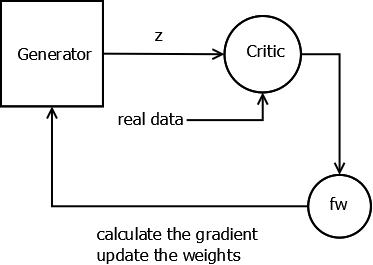
\includegraphics[scale=0.4]{media/WGAN.png}
	\caption{WGAN Architecture.} 
	\label{fig:wgan}
\end{figure}

